\mode*
\mode<article|presentation>{%
  \iftagged{handout-tufte}%
  {\section[Objetivos]{\textbf{\textcolor{blueun}{Objetivo general y objetivos espec\'ificos}}}}
  {\section[Objetivos]{Objetivo general y objetivos espec\'ificos}}
}
\label{sec:objs}
\mode<presentation>{
  \begin{frame}[label=objetivos]
    \objetivosTime
    \frametitle{Qu\'e se busca con esta investigaci\'on?}
    \begin{center}
      \LARGE \textbf{\textcolor{blueun}{Objetivo General y Objetivos Espec\'ificos}}
    \end{center}  
  \end{frame}
}
\mode<article|presentation>{%
  \iftagged{handout-tufte}%
  {\subsection[General]{\textbf{Objetivo general}}}
  {\subsection[General]{Objetivo general}}
}%
\label{sec:objgen}
\mode<presentation>{
  \begin{frame}<1-2>[label=def_objetivos]
    \defObjetivosTime
    \frametitle{Qu\'e se busca con esta investigaci\'on?}
    \textbf{\textcolor{blueun}{OG:}} Desarrollar un \alert<2>{marco de experiementaci\'on}\only<2-2>{\footnote{Marco o framework de investigaci\'on}}, mediante el cual se pueda implementar las hip\'otesis de soluci\'on de \alert<3>{los problemas de locomoci\'on}\only<3-3>{\footnote{Problemas actuales de robotica b\'ipeda}} de la rob\'otica subactuada y de caminadores.\\
    \hyperlink<2>{def_framework}{\beamergotobutton{Definici\'on de Framework}}
    \hyperlink<3>{def_problema}{\beamergotobutton{Problemas de locomoci\'on}}
  \end{frame}
  % Marco de Experimentaci\'on:
  % Es un aparato de conocimiento din\'amico con ejemplos construidos de plataformas b\'ipedas rob\'oticas que siguen los siguientes pasos
  % 1) Selecci\'on de plataforma: Que se quiere investigar o proponer? Que se quiere resolver? Que se quiere mejorar?
  % 2) Dise\~no mecanico: Planos, ensambles, elementos estandar, tipo de fabricaci\'on y presupuesto aproximado.
  % 3) Dise\~no electronico: Esquem\'aticos, PCBs(DIP,SMT), selecci\'on de microprecesadores, microcontroladores, sensores, actuadores y presupuesto aproximado.
  % 4) Sistema distribuido: Implementaci\'on red de sensores-actuadores, linux embebido, puesta en marcha y configuraci\'on del sistema distruibuido.
  % 5) Capa de aplicaciones: Selecci\'on de librer\'ias, implementaci\'on en un lenguaje de alto nivel de las estrategias de control y cognicion.
  \begin{frame}[plain,t,label=def_framework]
    \defFrameworkTime
    \hspace*{-0.8cm}\parbox[t]{\textwidth}{
      \only<1->{\vspace*{-0.4cm}\hspace*{-1.5cm}
        \colorbox{blueun}{
          \parbox[t][1.5cm][c]{\paperwidth}{
            \textcolor{white}{\Large\quad{MARCO DE EXPERIMENTACI\'ON}}
          }
        }
      }\vspace{0.05cm}\\
      \only<2>{\alert<2>{Framework o marco de experimentaci\'on se define en esta propuesta como:}}\\
      \only<3->{\alert<3>{Un aparato de conocimiento din\'amico con ejemplos construidos de plataformas b\'ipedas rob\'oticas que siguen los siguientes pasos.}}
      \only<3->{\small
        \begin{columns}[t] %¡Columnas como en TeX normal!
          \begin{column}{7cm}
            \begin{enumerate}
            \item<4-|alert@4,5> \hyperlink{def_framework<5>}{\textbf{Selecci\'on de plataforma\only<5-6>{:}} \only<5-6>{\scriptsize Qu\'e se quiere investigar o proponer? Qu\'e se quiere resolver? Qu\'e se quere mejorar?}}
            \item<4-|alert@4,7> \hyperlink{def_framework<7>}{\textbf{Dise\~no mec\'anico\only<7-8>{:}} \only<7-8>{\scriptsize Planos, ensambles, elementos estandar, tipo de fabricaci\'on y presupuesto aproximado.}}
            \item<4-|alert@4,9> \hyperlink{def_framework<9>}{\textbf{Dise\~no electr\'onico\only<9-10>{:}} \only<9-10>{\scriptsize Esquem\'aticos, ensambles, elementos estandar, tipo de fabricaci\'on y presupuesto aproximado.}}
            \item<4-|alert@4,11> \hyperlink{def_framework<11>}{\textbf{Sistema embebido y distribuido\only<11-12>{:}} \only<11-12>{\scriptsize Implementaci\'on de red, GNU-Linux embebido, puesta en marcha y configuraci\'on.}}
            \item<4-|alert@4,13> \hyperlink{def_framework<13>}{\textbf{Aplicaciones\only<13-14>{:}} \only<13-14>{\scriptsize Selecci\'on de librerias, lenguaje de alto nivel, implementaci\'on estrategias de control y congnici\'on.}}
            \end{enumerate}
          \end{column}
          \begin{column}{3cm}
            \\% espacio para ajustar las graficas
            \includegraphics<6>[height=4.0cm,width=3.0cm]{../images/TiposDePlataformas.png}
            \includegraphics<8>[height=4.0cm]{../images/DisenoMecanico.png}
            \includegraphics<10>[height=4.0cm]{../images/DisenoElectronico.png}
            \includegraphics<12>[height=4.0cm,width=3.5cm]{../images/DisenoEmbebidos.png}
            \only<14>{%
              \begin{itemize}\scriptsize
              \item C/C++
              \item Matlab-Sim-Mechanics
              \item OpenHRP3
              \item Open Dynamics Engine ODE
              \item Box2d
              \item PhysX
              \end{itemize}
            }%\includegraphics<9>[height=4.0cm]{../images/TODDLE-MIT.png}
          \end{column}
        \end{columns}
      }\vspace{0.5cm}
      \hyperlink<4->{def_objetivos<2>}{\beamerreturnbutton{Volver al Objetivo General}}
    }
  \end{frame}
  \againframe<3>{def_objetivos}
  \begin{frame}[label=objgen]
    \objgenTime
    \frametitle{Qu\'e se quiere lograr con esta investigaci\'on?}
    \framesubtitle{Framework de investigaci\'on y desarrollo de rob\'otica b\'ipeda}
    \begin{center}
      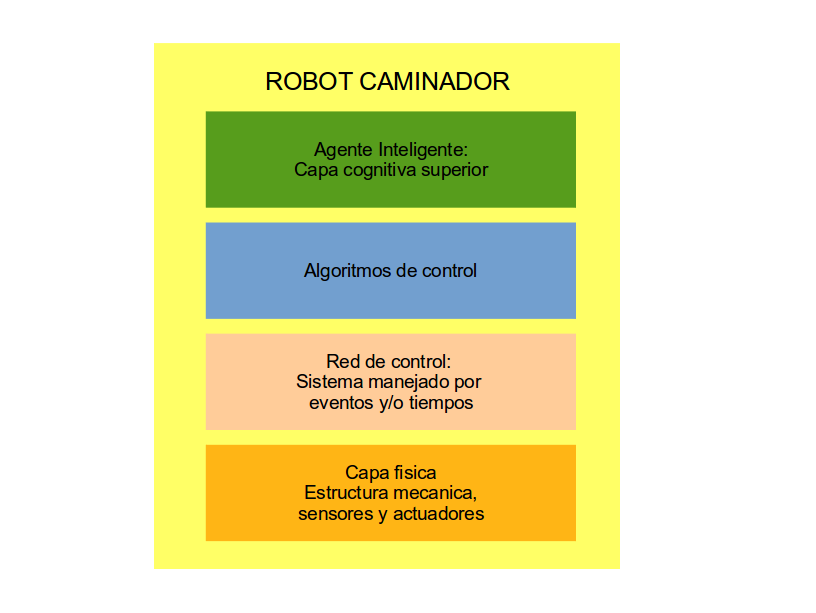
\includegraphics[height=7.0cm]{../images/objGen.png}
    \end{center}
  \end{frame}
}
\tagged{handout-tufte}{
  \begin{marginfigure}[-8.5cm]
    \centering
    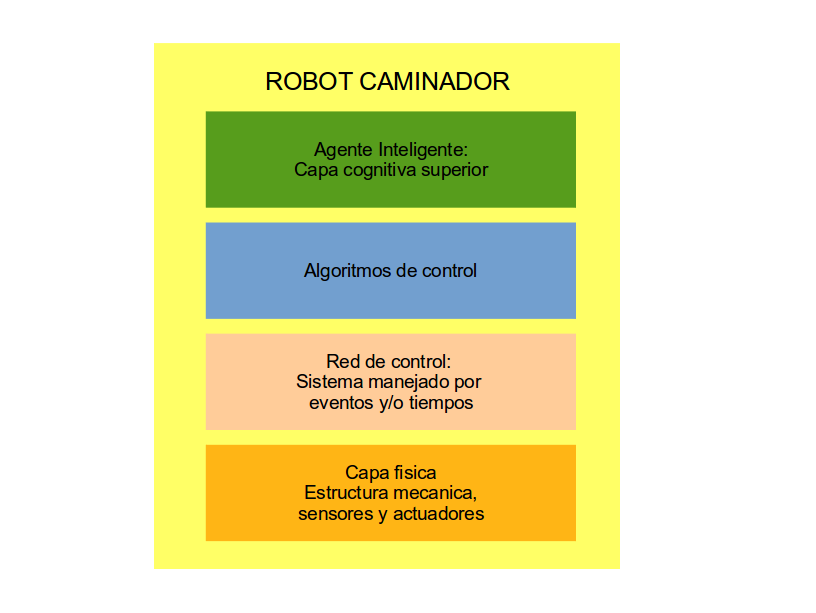
\includegraphics{../images/objGen.png}
    \caption{Objetivo General}
    \label{fig:objGen}
  \end{marginfigure}
}
\untagged{handout-tufte}{El principal objetivo de esta investigaci\'on se describe de forma global y gr\'afica en la Figura \ref{fig:objGen}, y es enunciado a continuaci\'on:\par}
\textbf{OG:} Dise\~nar y construir un \emph{\textbf{marco de experimentaci\'on}}\iftagged{handout-tufte}{%
  \sidenote[][-2.2cm]{\textbf{Marco de Experimentaci\'on:}
    {\scriptsize Es un aparato de conocimiento din\'amico con ejemplos construidos de plataformas b\'ipedas rob\'oticas que siguen los siguientes pasos:}
    \begin{enumerate}\tiny
    \item Selecci\'on de plataforma
    \item Dise\~no mecanico
    \item Dise\~no electronico 
    \item Sistema distribuido
    \item Capa de aplicaciones
    \end{enumerate}
  }
}{\footnote{compuesto por el dise\~no de una red de sensores-actuadores distribuida y un conjunto de dise\~no de eslanbones y articulaciones modulares para ser frabricados mediante prototipado r\'apido}} mediante el cual se pueda implementar\footnote{estudiar, proponer y/o comprobar} las hip\'otesis que solucionen los \emph{\textbf{problemas de locomoci\'on}}\iftagged{handout-tufte}{%
  \sidenote{\textbf{Problemas de la robotica b\'ipeda:}
    {\scriptsize Estan relacionados con el uso eficiente de la energ\'ia, la din\'amica pasiva de caminadores, presentes en:}
    \begin{enumerate}\tiny
    \item Estructuras mec\'anicas 
    \item Capa sensora y de actuaci\'on
    \item Control 
    \item Plan. y gen. de trayectorias 
    \item Capa de cognitiva
    \end{enumerate}
  }
}{\footnote{que permita la b\'usqueda de estructuras mecatr\'onicas eficientes energ\'eticamente, capaces de lograr la locomoci\'on requerida por las necesidades fundamentales de los robots caminadores}} de la rob\'otica subactuada y de caminadores\iftagged{handout-tufte}{ (Ver Figura. \ref{fig:objGen})}{}.\par
\untagged{handout-tufte}{
  \begin{figure}[!htb]
    \centering
    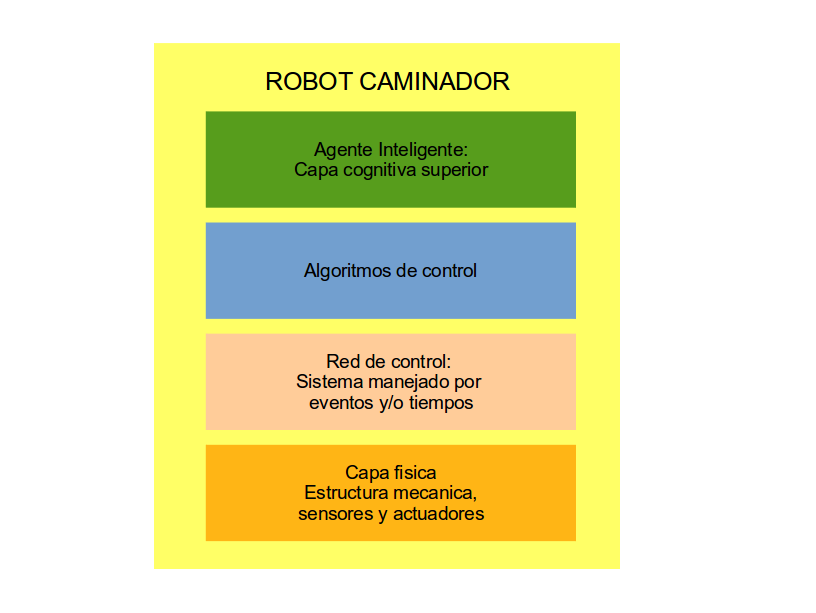
\includegraphics[scale=0.5]{../images/objGen.png}
    \caption{Objetivo General}
    \label{fig:objGen}
  \end{figure}
}

\mode<article|presentation>{%
  \iftagged{handout-tufte}%
  {\subsection[Especificos]{\textbf{Objetivos espec\'ificos}}}
  {\subsection[Especificos]{Objetivos especificos}}
}%
%\subsection[Especificos]{\iftagged{handout-tufte}{\textbf{Objetivos espec\'ificos}}{Objetivos espec\'ificos}}
\label{sec:objesp}
\mode<presentation>{
  \begin{frame}[label=def_objesp]
    \defObjespTime
    \frametitle{Qu\'e se requiere y qu\'e se obtiene para el Obj. Gen?}
    \framesubtitle{Algunos logros requeridos para el objetivo principal}
    \begin{center}
      \hyperlink{exp_capas<2>}{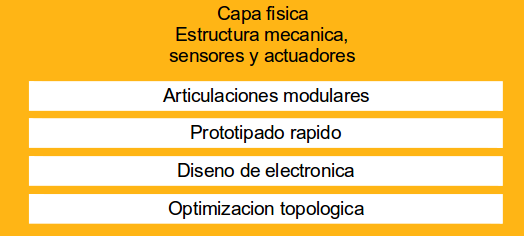
\includegraphics[height=2.0cm]{../images/objCapaFisica.png}}
      \hyperlink{exp_capas<3>}{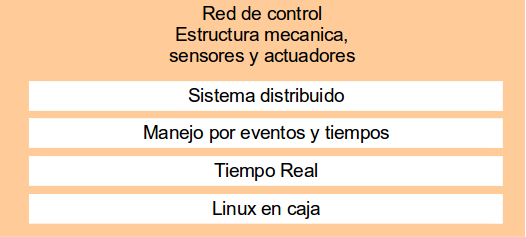
\includegraphics[height=2.0cm]{../images/objCapaRAS.png}}\\
      \hyperlink{exp_capas<4>}{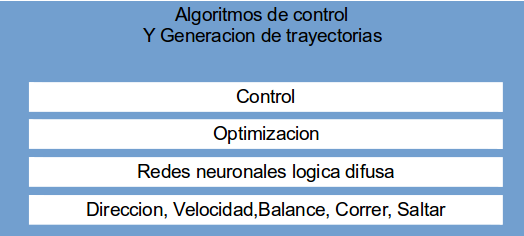
\includegraphics[height=2.0cm]{../images/objCapaControl.png}}
      \hyperlink{exp_capas<5>}{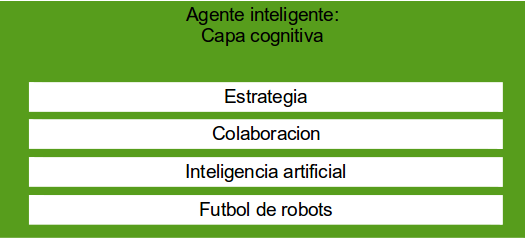
\includegraphics[height=2.0cm]{../images/objCapaCognitiva.png}}
    \end{center}
    \hyperlink{exp_capas}{\beamergotobutton{Explicaci\'on de Capas}}
  \end{frame}
}
\begin{enumerate}[\textbf{OE:} 1.]\tagged{handout-tufte}{\small}
\item Modelar, simular, analizar y sintetizar mecanismos subactuados que optimicen la energ\'ia para la locomoci\'on de caminar, saltar o correr.\untagged{handout-tufte}{\par}
\item Dise\~nar y construir una plataforma rob\'otica modular modular y para prototipado (ver Figura \ref{fig:objCapas} Capa Física), capaz de configurar cadenas cinem\'aticas  controladas y/o monitoreadas bajo el sistema distribuido\untagged{handout-tufte}{.\par}
\item Implementar un sistema distribuido de sensores y actuadores que funcione en tiempo-real  (ver Figura \ref{fig:objCapas} Capa de sensorial y de Actuaci\'on), bajo el principio de manejo por disparo-de-eventos y/o manejo por disparo-por-tiempos\untagged{handout-tufte}{\cite{Kimm2012}}.\par
\item Dise\~nar, simular e implementar diferentes controles de locomoci\'on (ver Figura \ref{fig:objCapas} Capa de control de locomoci\'on) inspirados en las nuevas tendencias de investigaci\'on de caminadores sobre plataformas rob\'oticas modulares construidas.\par
\item Dise\~nar, simular e implementar estrategias y actividades colaborativas usando una red de caminadores  (ver Figura \ref{fig:objCapas} Capa Cognitiva.).\par
\end{enumerate}
\iftagged{handout-tufte}{
  \begin{marginfigure}[-9.0cm]
    \centering
    %\parbox{11.6cm}{
      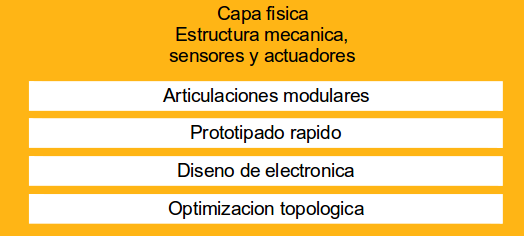
\includegraphics[width=5.0cm]{../images/objCapaFisica.png}\\
      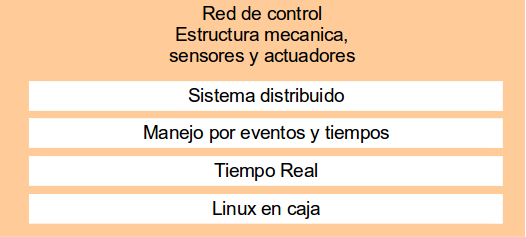
\includegraphics[width=5.0cm]{../images/objCapaRAS.png}\\
      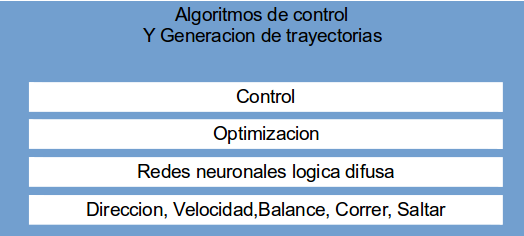
\includegraphics[width=5.0cm]{../images/objCapaControl.png}\\
      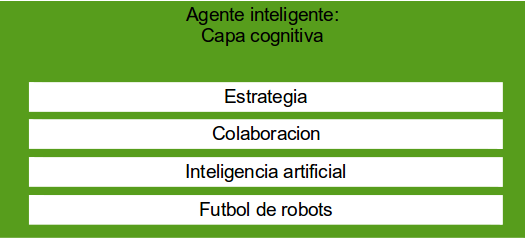
\includegraphics[width=5.0cm]{../images/objCapaCognitiva.png}
    %}\\
    \caption{Objetivos Específicos}
    \label{fig:objCapas}
  \end{marginfigure}
}{\begin{figure}[!htb]
    \centering
    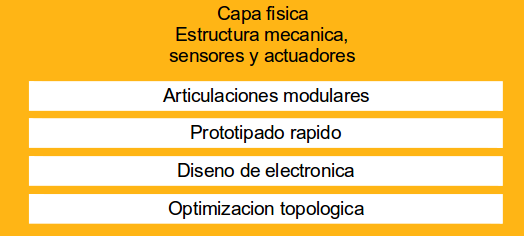
\includegraphics[scale=0.45]{../images/objCapaFisica.png}
    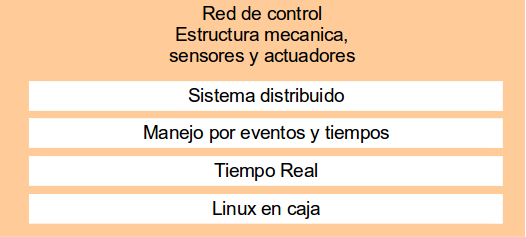
\includegraphics[scale=0.45]{../images/objCapaRAS.png}\\
    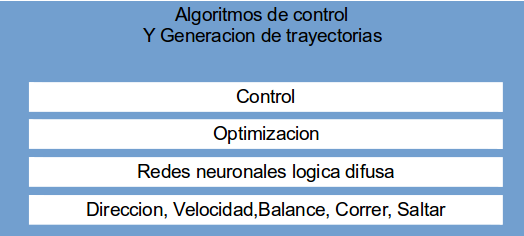
\includegraphics[scale=0.45]{../images/objCapaControl.png}
    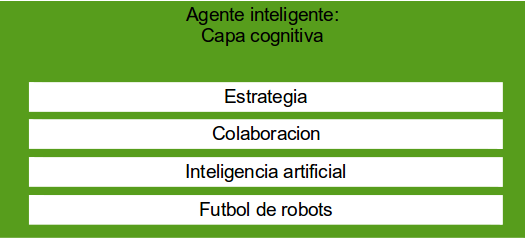
\includegraphics[scale=0.45]{../images/objCapaCognitiva.png}
    \caption{Objetivos Específicos}
    \label{fig:objCapas}
  \end{figure}
}